\chapter{METHODOLOGY}

\section{Introduction}

\hs This chapter describes the experimental design, data acquisition, model development, and evaluation procedures implemented during the internship project. The primary objective is to develop a robust and deployable deep learning framework for the automatic detection and pixel-level segmentation of cracks in large-scale, high-resolution aerial imagery captured by Unmanned Aerial Vehicles (UAVs) \cite{zhang-2024a, chen-2024}. The methodology has been designed to address the key technical objectives established in Chapter 1:

\begin{itemize}
    \item \textbf{Unify and standardize multiple public crack datasets} to construct a diverse and balanced data pool for model training.
    \item \textbf{Develop and evaluate multiple state-of-the-art architectures} across semantic segmentation, instance segmentation, and transformer-based paradigms.
    \item \textbf{Design and implement a tile-based inference pipeline with blended overlaps} to enable the seamless processing of arbitrarily large-scale images on a single Graphics Processing Unit (GPU).
    \item \textbf{Validate the pipeline on a custom, high-resolution self-collected UAV dataset} to verify its real-world robustness.
\end{itemize}

\section{Data Acquisition and Preparation}

\hs To train a robust and generalizable deep learning model, a diverse collection of data is required. This section details the curation of public benchmarks, the collection protocol of our custom UAV dataset, and the preprocessing steps established to unify these disparate sources.

\subsection{Public Datasets}
\label{subsec:public-datasets}

\hs To build a diverse and robust training corpus, we aggregated publicly available crack detection datasets curated in the GitHub repository \textbf{Cv-learning/Crack-Dataset}. This repository consolidates multiple benchmark datasets from the literature, providing a unified collection of crack images with corresponding pixel-level annotations.

\hs The combined dataset comprises 8,818 RGB images and their binary segmentation masks, covering a wide variety of crack morphologies, surface materials (concrete, asphalt, brick, etc.), and imaging conditions (different lighting, shadows, and viewing angles). The specific datasets included in this aggregation are those listed in the repository’s documentation, which bring together well-known benchmarks such as CFD, Crack500, DeepCrack, Tunnel Crack, and other sources as indicated in the repository. All images were resampled to a consistent resolution and paired with their ground-truth masks.

\begin{table}[htbp]
    \centering
    \setlength{\tabcolsep}{5pt}
    \caption{Detailed specifications of the constituent public crack datasets.}
    \label{tab:constituent_datasets}
    \begin{tabularx}{\textwidth}{l l X X}
        \toprule
        \textbf{Dataset}      & \textbf{Images} & \textbf{Surface}                   & \textbf{Academic Citation}             \\
        \midrule
        \textbf{CFD}          & 118             & Asphalt pavement                   & Shi et al. (2016) \cite{shi-2016}      \\
        \addlinespace
        \textbf{Crack500}     & 500             & Concrete pavements                 & Zhang et al. (2016) \cite{zhang-2016}  \\
        \addlinespace
        \textbf{DeepCrack}    & 537             & Cement, asphalt, and concrete      & Liu et al. (2019) \cite{liu-2019}      \\
        \addlinespace
        \textbf{Tunnel Crack} & \textbf{7,663}  & Concrete tunnel walls              & CV-learning Repository\footnotemark[1] \\
        \midrule
        \textbf{Total}        & \textbf{8,818}  & \textbf{Mixed structural surfaces} & \textbf{Combined Dataset}              \\
        \bottomrule
    \end{tabularx}
\end{table}

\footnotetext[1]{Retrieved from: \url{https://github.com/Cv-learning/Crack-Dataset}.}

\subsection{Planned Self-Collected UAV Dataset}

\hs To complement the public benchmarks with real-world aerial imagery, a custom UAV-based crack dataset was proposed for collection by the Drone Operations Department at AI Farm Robotics. The intended acquisition protocol specified flights at an altitude of 10–15 m using a high-resolution RGB sensor, targeting building facades and rooftops in Phnom Penh, with annotations to be performed manually by trained technicians.

\hs However, at the time of this internship (July–September 2026), the data collection and annotation pipeline had not been completed by the Drone Operations Department. Consequently, this dataset was not available for integration into the training, validation, or testing phases of the current study.

\hs The absence of this dataset does not invalidate the experimental framework, as the aggregated public datasets (Section~\ref{subsec:public-datasets}) provide a sufficiently diverse and challenging benchmark covering multiple surface types, lighting conditions, and crack morphologies. Validation on genuine UAV-captured imagery remains an important direction for future work, contingent on the completion of the data collection effort by the drone team.

\subsection{Annotation Unification and Standardization}

\hs To make all training data compatible, the annotation formats from different sources were converted into a common binary pixel representation. Each ground-truth label was transformed into a single-channel mask, where the mathematical definition is:

\begin{equation}
    M(x, y) = \begin{cases}
        1, & \text{if pixel } (x, y) \text{ belongs to a crack region} \\
        0, & \text{otherwise (background)}
    \end{cases}
\end{equation}

\hs For practical storage, these binary masks were saved as 8-bit single-channel PNG files. In this format, a pixel value of \textbf{255 (white)} represents a crack, corresponding to the mathematical value $1$, while a pixel value of \textbf{0 (black)} represents the background, corresponding to the mathematical value $0$. During data loading, the pixel values are normalized by dividing by 255 to recover the $\{0,1\}$ representation used for model training and loss computation. This dual representation, mathematical $\{0,1\}$ for computation and $\{0,255\}$ for storage, is standard practice in image segmentation and ensures compatibility with both deep learning frameworks and standard image I/O libraries.

\begin{figure}[htbp]
    \centering
    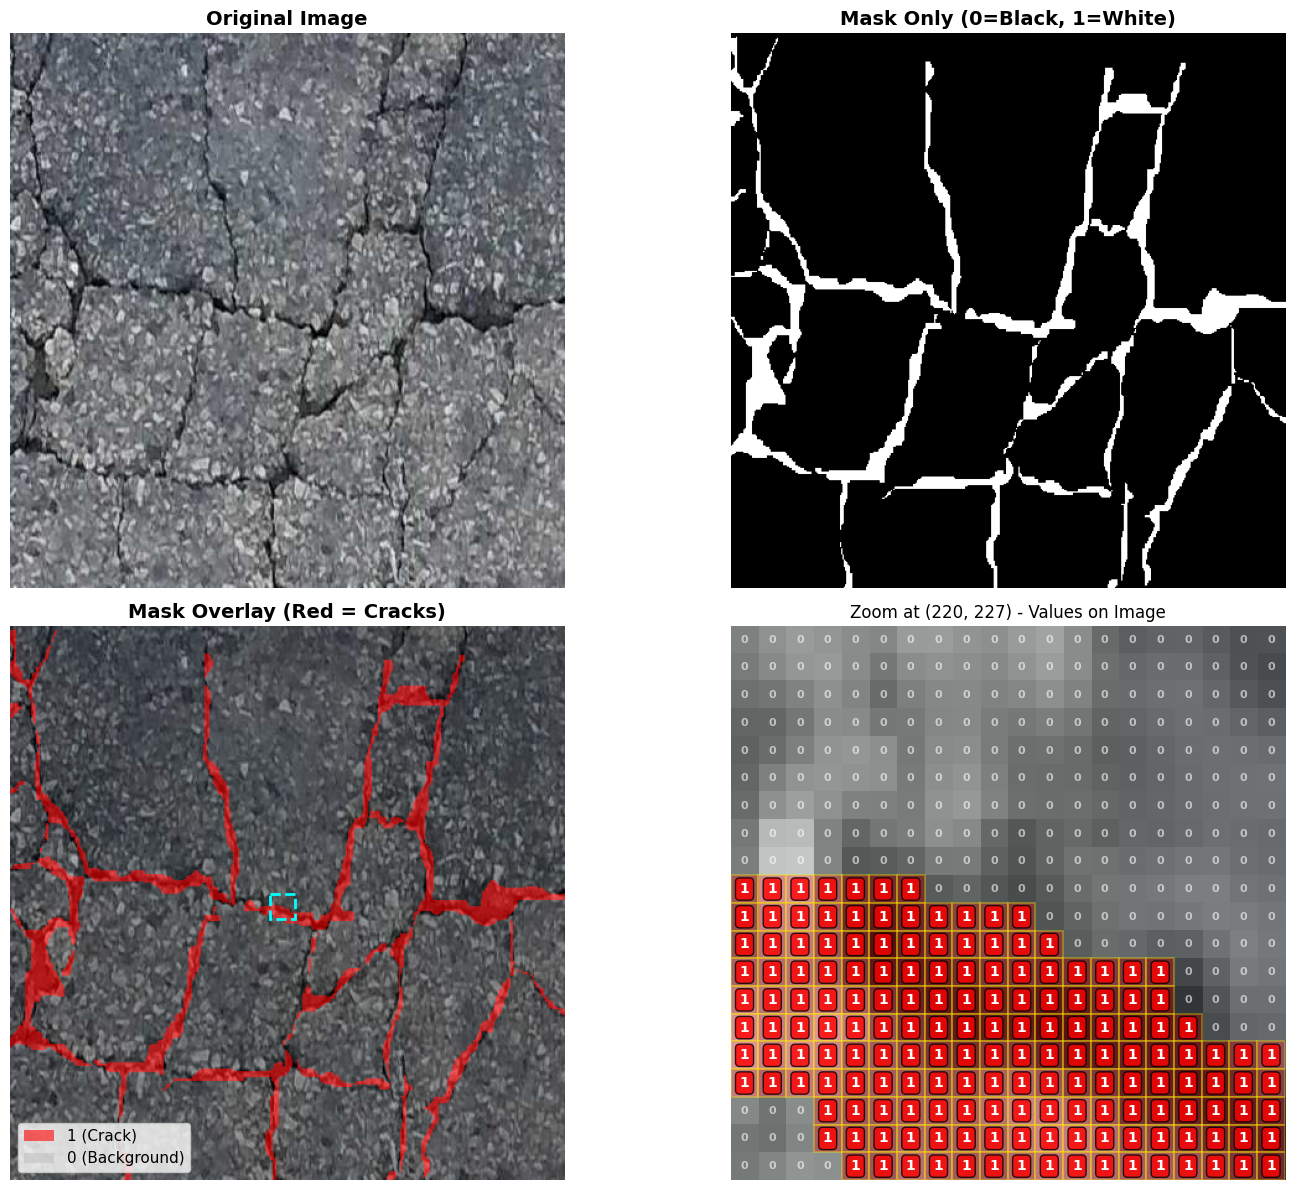
\includegraphics[width=\linewidth]{figures/cracks/crack-map.png}
    \caption{\textit{Binary pixel-level annotation used for model training and evaluation.}}
    \label{fig:crack_map}
\end{figure}

\hs This unified annotation scheme ensures consistent processing across all datasets. The binary representation simplifies loss computation and metric calculation while preserving pixel-level spatial precision.

\subsection{Patch Extraction and Sliding Window Strategy}

\hs To accommodate images of varying resolutions within a unified training and inference pipeline, all source images and their corresponding binary masks were decomposed into fixed-size tiles of \(512 \times 512\) pixels.

\textbf{Training Phase}

\hs All training images were sourced exclusively from the public crack datasets described in Section~\ref{subsec:public-datasets}. These images have a native resolution of \(448 \times 448\) pixels. To standardize inputs for batch processing, symmetric zero-padding was applied to the boundaries to reach the target size of \(512 \times 512\) pixels, as illustrated in Figure~\ref{fig:training_image_resize}. This padding ensures that the spatial aspect ratio is preserved without distorting the crack features.

\begin{figure}[htbp]
    \centering
    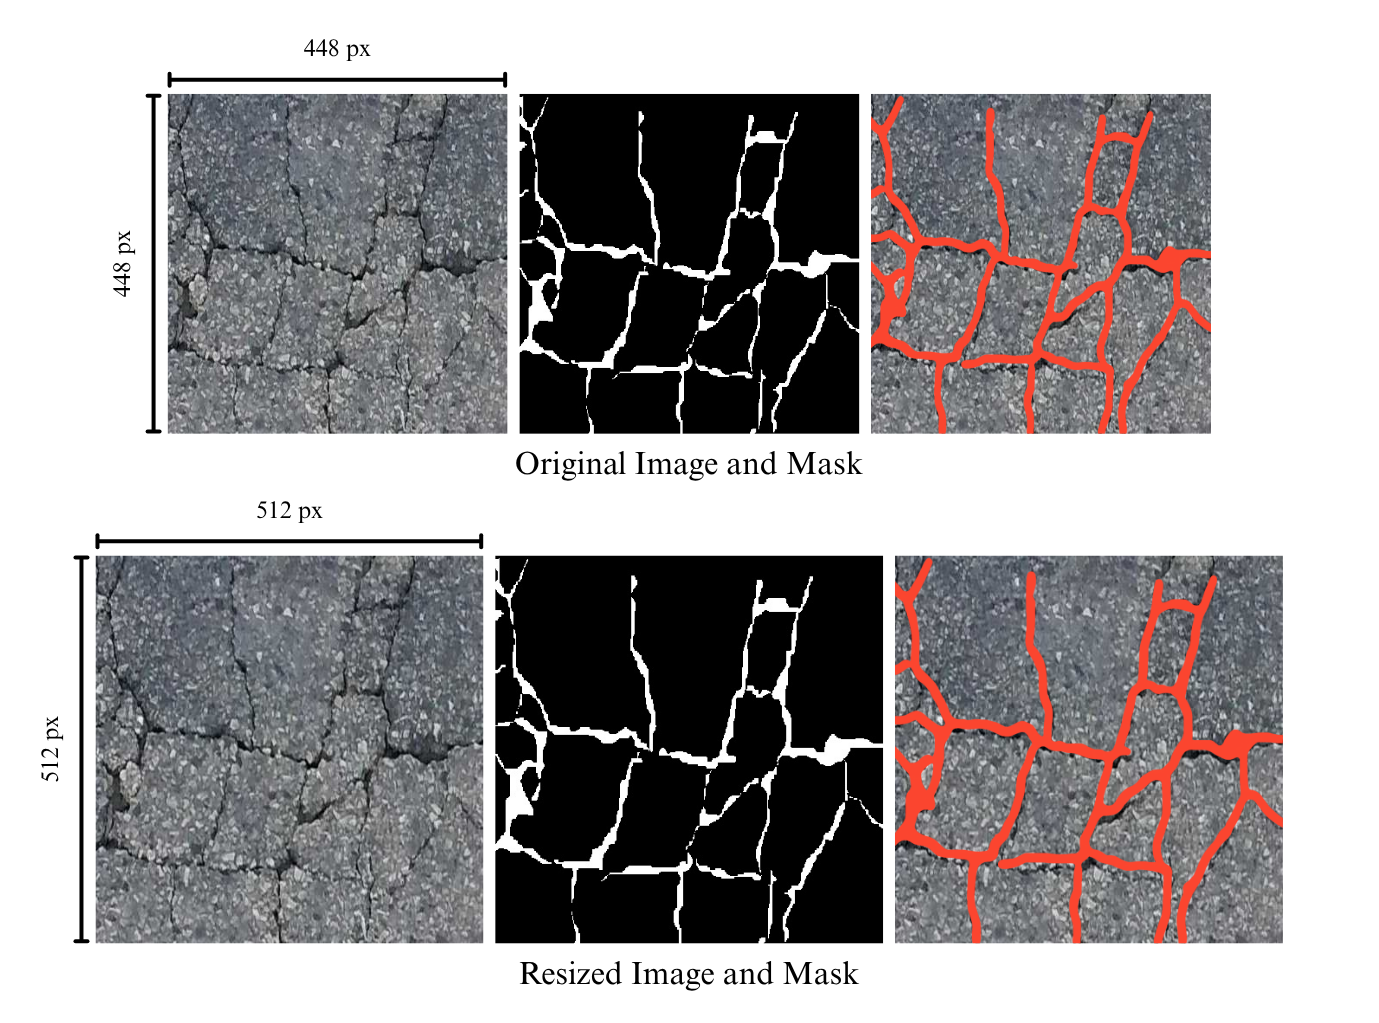
\includegraphics[width=\linewidth]{figures/cracks/image-resizing.png}
    \caption{\textit{Padding for training images, showing the symmetric zero-padding applied to reach the target size of \(512 \times 512\) pixels.}}
    \label{fig:training_image_resize}
\end{figure}

\textbf{Inference Phase}

\hs For high-resolution inference, the sliding window strategy was designed to process arbitrarily large images that exceed GPU memory limits. The window size was set to \(512 \times 512\) pixels with a stride of 384 pixels, corresponding to a 128-pixel overlap (25\%) in both horizontal and vertical directions.

\begin{figure}[htbp]
    \centering
    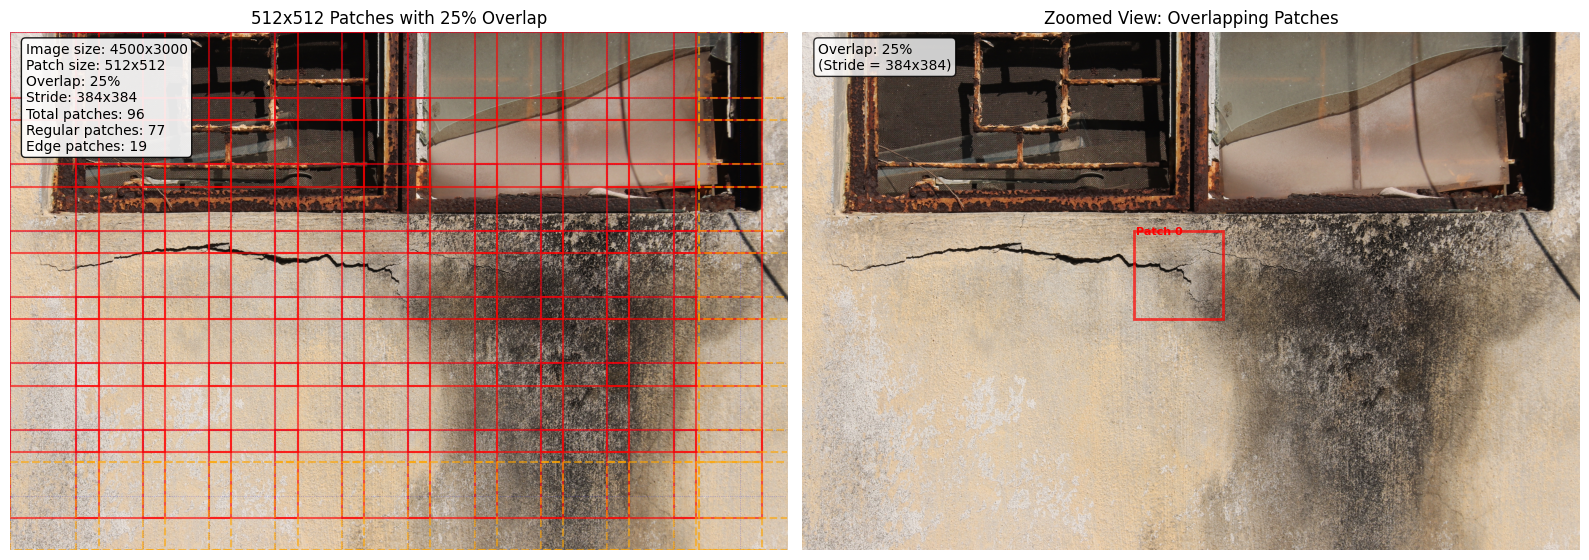
\includegraphics[width=\linewidth]{figures/cracks/inference-patching.png}
    \caption{\textit{Sliding window for high-resolution inference, showing the overlap between adjacent patches.}}
    \label{fig:inference_patching}
\end{figure}

\hs This overlap ensures that cracks located near tile boundaries are not truncated or lost during independent tile forward passes.

\hs \hl{The inference pipeline was validated on high-resolution test images of approximately 13.5 megapixels,} which were sourced from the public datasets' test split (where native resolutions exceeded \(512 \times 512\)) and used exclusively for evaluation. These images, while not reaching the gigapixel scale targeted for final deployment, were sufficiently large to demonstrate the effectiveness of the tile-based approach and the blended overlap merging strategy. The pipeline is architecturally scalable to gigapixel images, as the tile processing is independent of total image dimensions, requiring only sufficient disk storage and sequential processing.

\hs \hl{If an input image's dimensions are not perfectly divisible by the stride, zero-padding is temporarily applied to the right and bottom boundaries. After the blended overlap merging reconstructs the full probability map, the padded regions are cropped back to the original image dimensions.}

\begin{table}[h]
    \centering
    \caption{Summary of patch extraction and sliding window parameters}
    \label{tab:patch_parameters}
    \renewcommand{\arraystretch}{1.1}
    \begin{tabular}{@{}l c@{}}
        \toprule
        \textbf{Parameter}                     & \textbf{Value}            \\
        \midrule
        Training image size (before padding)   & \(448 \times 448\) pixels \\
        Training patch size (after padding)    & \(512 \times 512\) pixels \\
        Testing image size (before extraction) & <10 megapixels            \\
        Inference patch size                   & \(512 \times 512\) pixels \\
        Inference overlap                      & 128 pixels (\(25\%\))     \\
        \bottomrule
    \end{tabular}
\end{table}

\subsection{Dataset Splitting}

\hs To ensure fair and unbiased evaluation, the entire set of 8,818 images was divided strictly at the image level into three disjoint subsets:

\begin{table}[htbp]
    \centering
    \caption{Summary of public crack dataset partition.}
    \label{tab:dataset_split}
    \renewcommand{\arraystretch}{1.1}
    \resizebox{\textwidth}{!}{%
        \begin{tabular}{lccc l}
            \toprule
            \textbf{Dataset Split} & \textbf{Split Percentage (\%)} & \textbf{Paired Image Count} & \textbf{Role in Training Pipeline}                 \\
            \midrule
            Training               & 80\%                           & 7,054                       & Active gradient optimization \& backpropagation    \\
            Validation             & 10\%                           & 882                         & Hyperparameter selection \& overfitting prevention \\
            Testing                & 10\%                           & 882                         & Independent, unseen benchmark evaluation           \\
            \midrule
            \textbf{Total}         & \textbf{100\%}                 & \textbf{8,818}              & \textbf{Comprehensive Compiled Public Database}    \\
            \bottomrule
        \end{tabular}%
    }
\end{table}

\hs By enforcing source-image level splitting, tiles from the same physical road section or lighting condition were prevented from appearing in both the training and evaluation splits, thereby ensuring the generalizability of the performance metrics.

\subsection{Class Imbalance Analysis}
\hs An analysis of pixel-level class distribution in the training set revealed significant class imbalance:

\begin{table}[h]
    \centering
    \caption{\hl{Class distribution in training split.}}
    \label{tab:class_distribution}
    \renewcommand{\arraystretch}{1.1}
    \begin{tabular}{@{}l r c@{}}
        \toprule
        \textbf{Class} & \textbf{Pixel Count} & \textbf{Percentage} \\
        \midrule
        Background     & \hl{1,617,843,456}        & \hl{99.41\%}             \\
        Crack          & \hl{9,597,056}            & \hl{0.59\%}              \\
        \bottomrule
    \end{tabular}
\end{table}

\hs \hl{This extreme imbalance (approximately 168:1 background-to-crack ratio) confirms the necessity of using evaluation metrics such as IoU, F1-Score, and Recall that are robust to class imbalance, rather than relying on pixel accuracy.}

\subsection{Data Augmentation Strategy}

\hs To improve model generalization and prevent overfitting on the limited training data, a series of augmentations was applied \hl{online} during training. Each augmentation was applied to both the RGB image and its corresponding binary mask to maintain spatial correspondence for geometric transforms.

\hs The augmentation strategy varied slightly across model families due to differences in the underlying training frameworks. All augmentations were applied only to the training split; the validation and test splits were left unaltered.

\textbf{For U-Net and SegFormer (SMP-based models):}

\begin{table}[h]
    \centering
    \caption{Data augmentation parameters for SMP-based models (U-Net and SegFormer).}
    \label{tab:augmentation_smp}
    \renewcommand{\arraystretch}{1.25}
    \small
    \begin{tabular}{@{}l l c@{}}
        \toprule
        \textbf{Augmentation} & \textbf{Parameters}                                                     & \textbf{Probability} \\
        \midrule
        Horizontal Flip       & -                                                                       & 0.5                  \\
        Vertical Flip         & -                                                                       & 0.5                  \\
        Rotation              & \(\pm 15^\circ\)                                                        & 0.5                  \\
        Shift-Scale-Rotate    & scale \(\pm 10\%\), rotation \(\pm 15^\circ\)                           & 0.5                  \\
        Brightness-Contrast   & brightness \(\pm 20\%\), contrast \(\pm 20\%\)                          & 0.5                  \\
        Color Jitter          & brightness \(\pm 10\%\), contrast \(\pm 10\%\), saturation \(\pm 10\%\) & 0.5                  \\
        Random Shadow         & shadow\_roi = (0, 0.5, 1, 1)                                            & 0.5                  \\
        Gauss Noise           & var\_limit = (10, 50)                                                   & 0.2                  \\
        Motion Blur           & blur\_limit = 5                                                         & 0.2                  \\
        \bottomrule
    \end{tabular}
\end{table}

\hs After augmentation, images were normalized using \textbf{ImageNet} mean [0.485, 0.456, 0.406] and standard deviation [0.229, 0.224, 0.225] as required by the pre-trained backbones.

\textbf{For YOLO (Ultralytics framework):}

\hs YOLO employs the native augmentation pipeline integrated within the Ultralytics framework. The default augmentations were used with the following parameters:

\begin{itemize}
    \item \textbf{HSV Augmentation}: Hue ($\pm$0.015), Saturation ($\pm$0.7), Value ($\pm$0.4)
    \item \textbf{Geometric}: Horizontal flip (p=0.5), Scale ($\pm$0.5)
    \item \textbf{Albumentations} (applied with lower probability): Blur, Median Blur, Grayscale conversion, CLAHE (Contrast Limited Adaptive Histogram Equalization)
\end{itemize}

\hs These augmentations are automatically applied during training and are optimized for the YOLO architecture's single-stage detection pipeline. No vertical flips, rotations, or photometric augmentations were applied to YOLO training as these are not included in the default Ultralytics segmentation augmentation configuration.

\section{Model Development and Selection}

\hs To empirically evaluate the trade-offs between accuracy, inference speed, and spatial context-awareness, three distinct families of state-of-the-art segmentation architectures were selected and evaluated.

\textbf{Selection Rationale}

The choice of architectures was guided by three primary considerations:

\begin{itemize}
    \item \textbf{Architectural diversity:} To compare fundamentally different approaches to segmentation (CNN-based semantic segmentation, CNN-based instance segmentation, and transformer-based segmentation).
    \item \textbf{Deployability:} All selected models are lightweight enough for edge-device deployment, a key requirement for the internship's focus on practical robotics applications at AI Farm Robotics.
    \item \textbf{Proven performance:} Each architecture has demonstrated strong performance on crack detection or similar fine-structure segmentation tasks in the literature.
\end{itemize}

\begin{table}[h]
    \centering
    \caption{Comparison of selected model architectures.}
    \label{tab:model_comparison}
    \renewcommand{\arraystretch}{1.2}
    \resizebox{\textwidth}{!}{%
        \begin{tabular}{@{}l l c c c@{}}
            \toprule
            \textbf{Model Family} & \textbf{Backbone} & \textbf{Params (M)} & \textbf{FLOPs (G)} & \textbf{Key Feature}                         \\
            \midrule
            U-Net                 & EfficientNet-B0   & 6.30                & 12.0               & Skip connections preserve fine crack details \\
            SegFormer             & MiT-B0            & 3.71                & 7.87               & Global receptive field via self-attention    \\
            YOLO                  & YOLO26s-seg       & 11.43               & 34.3               & Single-stage, instance-level output          \\
            \bottomrule
        \end{tabular}%
    }
\end{table}

\subsection{Baseline Architectures}

\subsubsection{Semantic Segmentation: U-Net}

\hs U-Net was selected as the primary semantic segmentation baseline due to its established performance in crack detection. The architecture employs a symmetric encoder-decoder structure with skip connections that directly transfer high-resolution local features from the encoder to the decoder. This design is particularly beneficial for thin crack detection, as it preserves fine spatial details that are often lost in deeper networks.

\begin{sloppypar}
    \hs The EfficientNet-B0 backbone was chosen as the encoder for its favorable trade-off between model size and representational capacity. With only \textbf{6.3 million parameters}, EfficientNet-B0 balances computational efficiency with strong feature extraction performance, making it suitable for deployment on resource-constrained edge devices. The U-Net decoder incorporates Spatial and Channel Squeeze-and-Excitation (scSE) attention to further refine feature representations and improve detection of subtle crack patterns.
\end{sloppypar}

\textbf{Strengths:} Superior preservation of fine spatial details; well-established performance on crack segmentation; computationally efficient.

\textbf{Weaknesses:} Limited global receptive field; may struggle with contextual understanding in complex scenes.

\subsubsection{Instance Segmentation: YOLO}

\hs \hl{YOLO was selected to evaluate whether treating distinct cracks as separate instances reduces noise and improves global delineation. The YOLO family of single-stage, anchor-free detectors is well-suited for real-time edge deployment due to its efficient architecture.}

\hs \hs{The YOLO26s-seg variant used in this study balances speed and accuracy, incorporating features such as Programmable Gradient Information (PGI) and the Generalized Efficient Layer Aggregation Network (GELAN) to retain spatial details while maintaining low latency. The model outputs both bounding boxes and pixel-level masks, enabling instance-wise analysis of individual cracks. With 11.4 million parameters and 34.3 GFLOPs, YOLO26s-seg is computationally heavier than the semantic segmentation models but offers the advantage of distinguishing individual crack instances.}

\textbf{Strengths:} Fast inference; instance-level differentiation; suitable for real-time edge deployment.

\textbf{Weaknesses:} May miss very thin cracks; requires careful threshold tuning; higher computational cost than lightweight semantic models.

\subsubsection{Transformer-Based Models: SegFormer}

\hs \hl{SegFormer was selected to evaluate the potential benefits of global receptive fields for crack detection. Traditional convolutional neural networks process features locally using fixed receptive fields, which can lead to loss of continuity for long, branching cracks. Transformers, in contrast, employ self-attention mechanisms to model long-range spatial dependencies across the entire image canvas.}

\hs \hl{The SegFormer architecture combines a hierarchical Mix Transformer (MiT) encoder with a lightweight MLP decoder. The MiT-B0 variant used in this study captures both high-resolution local details and global contextual features without requiring positional encodings, avoiding performance drops when test resolution differs from training resolution. With only \textbf{3.7 million parameters}, SegFormer-MiT-B0 is the lightest model evaluated in this study.}

\textbf{Strengths:} Global receptive field; preserves geometric continuity; lightweight.

\textbf{Weaknesses:} Lacks translational equivariance inductive bias; requires more training data; computationally expensive for self-attention at higher resolutions.

\subsubsection{Loss Functions}

\hs For U-Net and SegFormer (SMP-based models), a combined loss function was employed to address the extreme class imbalance inherent in crack detection, where crack pixels typically occupy less than 1\% of the total image area. The total loss is formulated as:
\begin{equation}
    L_{\text{total}} = w_{\text{BCE}} \cdot L_{\text{BCE}} + w_{\text{Dice}} \cdot L_{\text{Dice}} + w_{\text{Focal}} \cdot L_{\text{Focal}}
\end{equation}
where the three components are defined as follows.

\textbf{Binary Cross-Entropy (BCE) Loss.} BCE provides pixel-wise classification supervision, ensuring each pixel is individually evaluated against the ground truth:
\begin{equation}
    L_{\text{BCE}} = -\frac{1}{N} \sum_{i=1}^{N} \left[ y_i \log(p_i) + (1 - y_i) \log(1 - p_i) \right]
\end{equation}

\textbf{Dice Loss.} Dice loss optimizes the overlap between predicted and ground truth masks, which is more robust to class imbalance than BCE alone. It directly maximizes the F1-score at the pixel level:
\begin{equation}
    L_{\text{Dice}} = 1 - \frac{2 \, |P \cap G|}{|P| + |G|}
\end{equation}
where $P$ and $G$ denote the predicted and ground truth masks, respectively.

\textbf{Focal Loss.} Focal loss \cite{29-lin-2017} down-weights the contribution of well-classified examples, forcing the model to focus on hard-to-classify crack pixels:
\begin{equation}
    L_{\text{Focal}} = -\frac{1}{N} \sum_{i=1}^{N} (1 - p_i)^{\gamma} \, y_i \log(p_i)
\end{equation}
A focusing parameter of $\gamma = 2.0$ was used.

\textbf{For YOLO:} \hl{YOLO employs its native loss function as implemented in the Ultralytics framework. The loss comprises multiple components:}
\begin{equation}
    L_{\text{YOLO}} = L_{\text{box}} + L_{\text{cls}} + L_{\text{dfl}} + L_{\text{mask}}
\end{equation}
where:
\begin{itemize}
    \item $L_{\text{box}}$ is the bounding box regression loss (CIoU loss).
    \item $L_{\text{cls}}$ is the classification loss for object presence.
    \item $L_{\text{dfl}}$ is the Distribution Focal Loss for improved localization.
    \item $L_{\text{mask}}$ is the binary segmentation loss for mask prediction.
\end{itemize}

This multi-component loss enables YOLO to jointly optimize detection and segmentation in a single-stage pipeline.

\section{Implementation Details}

\hs The technical environment was built in mixed modes both digital and physical; it is a hybrid setup:

\textbf{Training Specifications:} The models were trained on Google Colab equipped with Tesla T4 GPU runtime with 16 GB of VRAM.

\textbf{Hardware Implementation:} During development, the models were implemented using intern's hardware, which has limited computational resources; however, the models were optimized to run efficiently within these constraints. \hl{Later on, the models were tested on a more powerful workstation with an NVIDIA RTX 4070 GPU from the company to validate performance and inference speed.}

\section{Evaluation Framework}
This section describes the quantitative evaluation metrics and the protocol established to compare the performance of different models.

\subsection{Evaluation Metrics}
\label{subsec:metrics}
Due to the extreme class imbalance in crack detection (where crack pixels typically occupy less than 1\% of the total image area), traditional pixel accuracy is highly misleading. A naive model predicting 100\% background would score $>99\%$ accuracy while failing completely. Therefore, the models are evaluated using metrics that focus on the positive class:
\begin{enumerate}
    \item \textbf{Intersection over Union (IoU):} Measures the ratio of overlapping area to union area between predicted mask $P$ and ground truth $G$:
          \begin{equation}
              \text{IoU} = \frac{|P \cap G|}{|P \cup G|} = \frac{\text{TP}}{\text{TP} + \text{FP} + \text{FN}}
          \end{equation}
    \item \textbf{Precision:} Measures the proportion of correctly predicted crack pixels among all predicted crack pixels:
          \begin{equation}
              \text{Precision} = \frac{\text{TP}}{\text{TP} + \text{FP}}
          \end{equation}
    \item \textbf{Recall:} Measures the proportion of correctly predicted crack pixels among all true crack pixels:
          \begin{equation}
              \text{Recall} = \frac{\text{TP}}{\text{TP} + \text{FN}}
          \end{equation}
    \item \textbf{F1-Score:} The harmonic mean of precision and recall, balancing false positives and false negatives:
          \begin{equation}
              \text{F1-Score} = \frac{2 \cdot \text{Precision} \cdot \text{Recall}}{\text{Precision} + \text{Recall}}
          \end{equation}
    \item \textbf{Inference Time:} Measured as the average processing time per Megapixel (seconds/MP) or Frames Per Second (FPS) on the target hardware to assess real-world deployability.
\end{enumerate}

\subsection{Baseline Comparisons}

\hs The performance of each trained architecture is compared against other evaluated models under the same unified protocol. To verify their competitiveness, the results are compared with state-of-the-art metrics published in the literature \cite{liu-2019, zhang-2024c, sohaib-2024}. The objective is to identify which model paradigm offers the optimal balance between pixel-level connectivity conservation, boundary precision, and latency, providing a solid reference for actual edge-device deployment.